\documentclass[aspectratio=169]{beamer}
\usetheme{Madrid}
\usecolortheme{owl}
\usepackage{graphicx} % Required for including images
\usepackage{amsmath} % Required for math equations

\title{HAYAL ET: An Interactive Theatrical Experience}
\subtitle{Exploring Choice, Consequence, and Reality}
\author{İpek Kennington}
%\institute{}
\date{\today}

\begin{document}

\frame{\titlepage}

\section{Project Overview}
\begin{frame}{Project Overview: What is HAYAL ET?}
    \begin{itemize}
        \item HAYAL ET (Imagine It) is an innovative interactive play that redefines the boundaries between traditional theatre and modern technology.
        \item It offers a dynamic narrative experience where the audience actively participates in shaping the story.
        \item The core idea is to explore the profound impact of choices and their subsequent consequences in a tangible, immersive way.
        \item Our goal is to create a deeply engaging and thought-provoking theatrical event that resonates uniquely with each audience member.
    \end{itemize}
\end{frame}

\section{The Core Concept}
\begin{frame}{The Core Concept: Branching Narratives \& Themes}
    \begin{itemize}
        \item \textbf{Branching Narrative:} The play features a multi-layered story with multiple deviation points. Audience decisions directly influence the plot's direction, leading to various unique paths and endings.
        \item \textbf{Themes Explored:}
        \begin{itemize}
            \item Choice \& Consequence: Every decision has a visible and immediate impact on the characters and the world.
            \item Nature of Reality: The play delves into questions about perception, reality, and the construction of personal experience.
            \item Moral Ambiguity: Scenarios are designed to present complex ethical dilemmas without easy answers.
        \end{itemize}
        \item \textbf{Audience as Co-authors:} The audience transitions from passive observers to active participants, co-creating the narrative journey.
    \end{itemize}
\end{frame}

\section{Technology \& Interaction}
\begin{frame}{Technology: The Interactive Engine}
    \begin{itemize}
        \item \textbf{Custom-Built System:} A bespoke software solution manages the complex web of narrative branches, character states, and environmental variables.
        \item \textbf{Audience Interaction Methods:}
        \begin{itemize}
            \item Mobile Interface: Audience members can use their smartphones (or provided devices) to vote on crucial decisions at key junctures.
            \item Real-time Data Processing: The system instantly processes collective audience input to determine the next scene or plot development.
            \item Dynamic Projection \& Sound: Visual and auditory elements of the play can change in real-time based on audience choices, enhancing immersion.
        \end{itemize}
        \item \textbf{Dynamic Progression:} The play's script and staging are designed to be flexible, allowing for seamless transitions between different narrative paths.
    \end{itemize}
\end{frame}
\begin{frame}{Mobile Interface: User Experience}
    \begin{figure}[h]
        \begin{minipage}{0.45\textwidth}
            \centering
            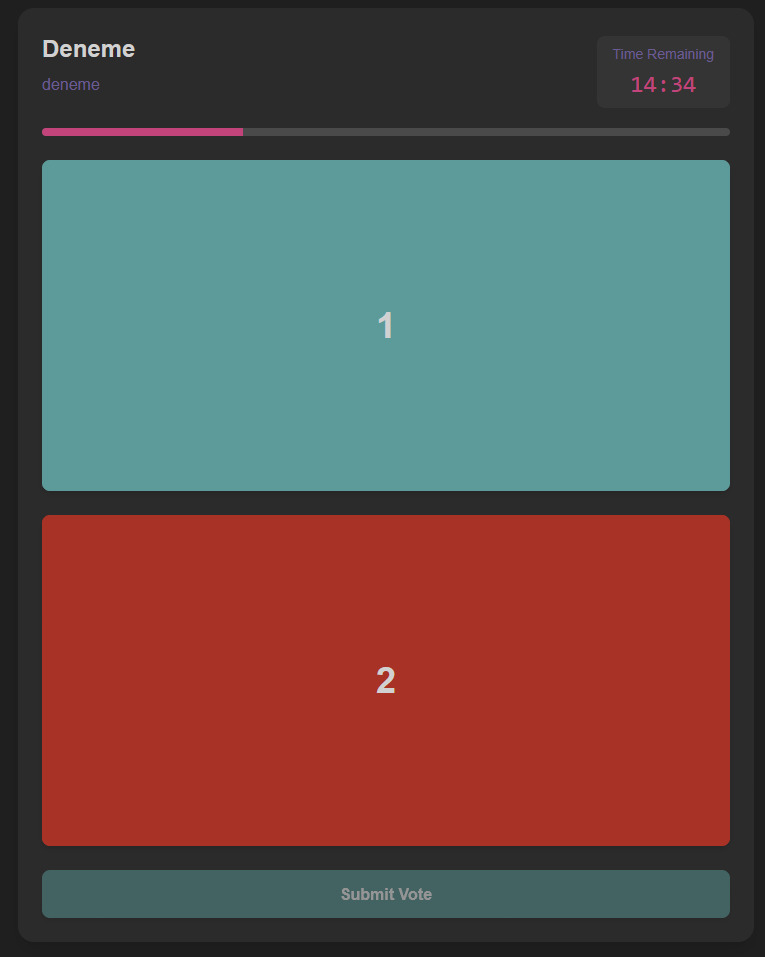
\includegraphics[height=0.7\textheight]{mobile_screen1.jpg}
            \caption{Audience voting interface}
        \end{minipage}
        \hfill
        \begin{minipage}{0.45\textwidth}
            \centering
            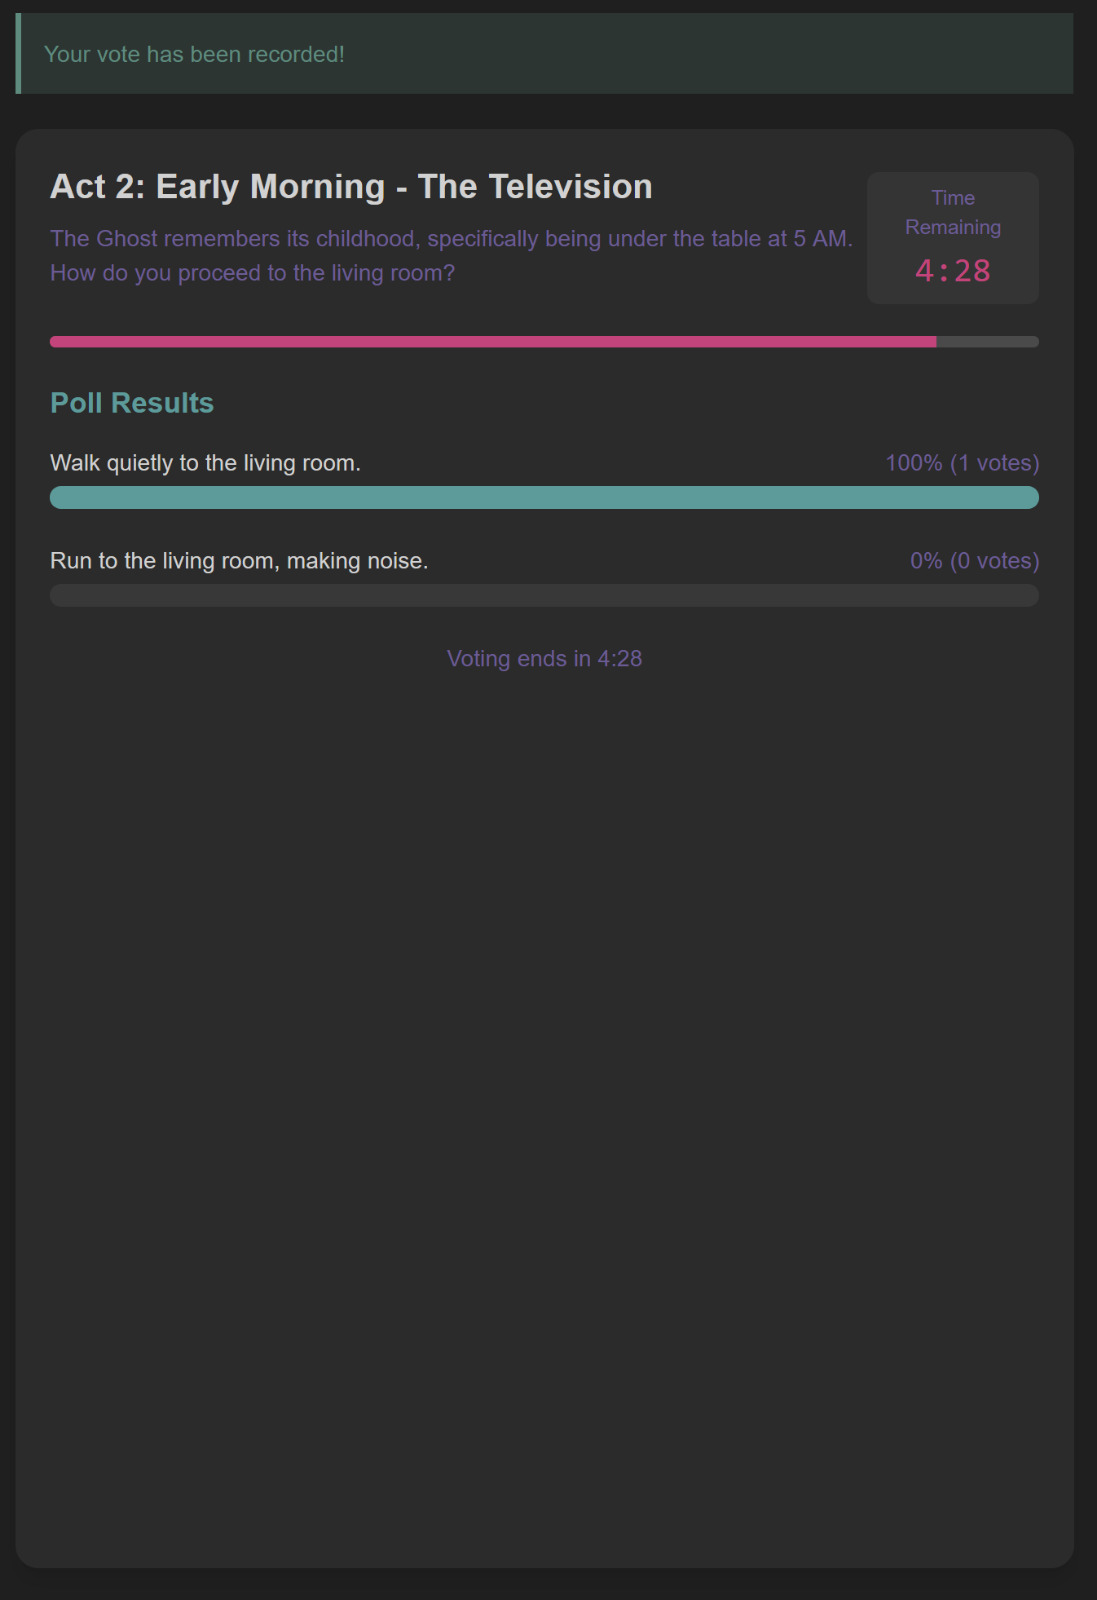
\includegraphics[height=0.7\textheight]{mobile_screen2.jpg}
            \caption{Results display screen}
        \end{minipage}
    \end{figure}
\end{frame}


\begin{frame}{Interaction Example: The Crossroads}
    Imagine the protagonist reaches a critical crossroads, facing two distinct paths:
    \begin{itemize}
        \item \textbf{Path A: The Path of Confrontation} - Leads to a direct and potentially dangerous encounter.
        \item \textbf{Path B: The Path of Evasion} - Offers a stealthier, but perhaps morally compromising, route.
    \end{itemize}
    The audience collectively decides which path the protagonist takes. The chosen path significantly alters the subsequent scenes, challenges, and character interactions.
\end{frame}


\section{Scenario Deep Dive: The Mysterious Box}
\begin{frame}{Scenario: The Enigmatic Artifact - Setup}
    \textbf{Setup:} In a pivotal scene, the main character discovers an old, ornate box. Its origins are unknown, and it emanates a faint, unsettling hum.
    \newline\newline
    \textbf{The Dilemma:} The character is faced with a choice:
    \begin{itemize}
        \item Open the box immediately, driven by curiosity and the potential for discovery (or peril).
        \item Leave the box untouched, fearing its unknown contents and potential negative consequences.
        \item Seek more information or tools before deciding, introducing a delay and potentially new variables.
    \end{itemize}
    \textbf{Audience Vote:} The audience is prompted to vote on one of these actions.
\end{frame}

\begin{frame}{Scenario: The Enigmatic Artifact - Consequences}
    \textbf{Potential Consequences (Illustrative):}
    \begin{itemize}
        \item \textit{Opening the Box:} Could reveal a vital clue, a dangerous trap, a source of power, or something entirely unexpected, leading to drastically different story branches.
        \item \textit{Leaving it:} Might lead to missed opportunities, a lingering sense of unease, or another character finding it later, altering their path.
        \item \textit{Seeking Information:} Could involve new scenes, dialogues with other characters, or the discovery of related lore, adding depth before returning to the decision with more context.
    \end{itemize}
\end{frame}

\section{Project Goals \& Target Audience}
\begin{frame}{Project Goals}
    \begin{itemize}
        \item To pioneer a new form of interactive storytelling in a live theatrical setting.
        \item To provide a highly personalized and replayable experience.
        \item To foster discussion and reflection on the themes of choice, agency, and determinism.
        \item To successfully integrate technology seamlessly into the performance without overshadowing the human element of theatre.
    \end{itemize}
\end{frame}

\begin{frame}{Target Audience}
    \begin{itemize}
        \item Theatre-goers looking for innovative and unconventional experiences.
        \item Individuals interested in interactive narratives, video games with strong storytelling, and escape rooms.
        \item Students and enthusiasts of drama, technology, and new media.
        \item Anyone curious about the intersection of art and technology.
    \end{itemize}
\end{frame}


\section{Conclusion \& Future Vision}
\begin{frame}{Conclusion: A Unique Theatrical Journey}
    \begin{itemize}
        \item HAYAL ET offers more than just a play; it's an experience, a conversation, and an exploration.
        \item By placing the power of choice in the hands of the audience, we create a performance that is both deeply personal and collectively shaped.
        \item We believe this approach to interactive theatre has the potential to engage audiences in unprecedented ways.
    \end{itemize}
\end{frame}

\begin{frame}{Future Vision}
    \begin{itemize}
        \item Explore different genres and narrative structures within the HAYAL ET framework.
        \item Enhance the technological backend for even more complex interactions and environmental responses.
        \item Develop tools and workshops to enable other creators to build their own interactive theatrical pieces.
        \item Potentially adapt the HAYAL ET concept for other mediums or educational purposes.
    \end{itemize}
\end{frame}

\end{document} 